\documentclass{article} % Tipo de documento

\usepackage[utf8]{inputenc} % Permite el uso de caracteres del Español

\usepackage[T1]{fontenc}

\usepackage{graphicx}

\usepackage{subfig}

% Carátula del Artículo  

\title{Reporte de Actividad 6}

\author{Brenda Leyva Amaya}

\date{19 de Marzo, 2018}
 

\begin{document}

\maketitle % Crea el título


\section{Introducción.}

En esta actividad se aborda el modelo de dos resortes acoplados con el fin de utilizar las funciones de jupyter lab para resolver las ecuaciones correspondientes y poder encontrar el comportamiento gráfico de estos resortes bajo diferentes circunstancias. Gracias a esta actividad nos acercamos a un jupyter mucho más útil para los diferentes ejercicios de modelado que se llevan a cabo en las áreas matemáticas y científicas. 

\section{Sistema de dos resortes acoplados.}

Texto de Temple H. Fay y Sarah Duncan Graham.

\vspace{0.5 cm}

En el artículo que se ha revisado se investiga el problema que aparece alejado de la discusión práctica para ser incluido únicamente como una descripción en los libros de texto. Esto es el problema de dos resortes con dos masas unidos en serie que cuelgan de un techo, en el cual se asume que las fuerzas restitutivas se comportan de acuerdo con la Ley de Hooke. Este problema se modela con un par de ecuaciones diferenciales lineales de segundo orden. 

\vspace{0.5 cm}

Se puede investigar cuando el movimiento de las dos masas está sincronizado o en fase y cuando se oponen entre sí o a 180 grados fuera de fase, esto se logra modificando las constantes de resorte. En el texto también se demuestra con ejemplos que algunos movimientos interesantes pueden surgir cuando una ligera no linealidad se introduce como un intento de incrementar las fuerzas restitutivas. 

\subsection{El modelo de resortes acoplados.}

El modelo consiste de dos resortes y dos masas. Con constantes de resorte k1 y k2 respectivamente, este se coloca a partir del techo y el peso de la masa m1 se une teniendo un resorte en su parte inferior al cual se le agrega la masa m2. Permitiendo que el sistema llegue a un punto de equilibrio, se mide el desplazamiento del centro de masa de cada una de las masas a partir del equilibrio como una función del tiempo y se denotan estas medidas como X1(t) y x2(t) respectivamente. 

\vspace{0.5 cm}

Se asume que las fuerzas restitutivas son de la forma -k1l1 y -k2l2 donde l1 y l2 son las elongaciones o compresiones de los dos resortes. Debido a que la masa superior esta unida a dos resortes, existen dos fuerzas restitutivas actuando sobre ella dadas por -k1x1 y -k2(x2-x1), mientras que la segunda masa solo siente la fuerza correspondiente a el segundo resorte. 

\subsection{Ejemplo 2.1.}
Se describe el movimiento de dos resortes con constantes k1=6 y k2=4 con condiciones iniciales (1,0,2,0) donde 1 y 2 son los desplazamiento y 0 y 0 son las velocidad iniciales. 

\vspace{0.5 cm}

** Resolución con jupyter lab de las ecuaciones correspondientes:

\begin{verbatim} 

# Use ODEINT to solve the differential equations defined by the vector field
from scipy.integrate import odeint
import numpy as np

# Parameter values

# Masses:
m1 = 1.0
m2 = 1.0

# Spring constants
k1 = 6.0
k2 = 4.0

# Natural lengths
L1 = 0.0
L2 = 0.0

# Friction coefficients
b1 = 0.0
b2 = 0.0

# Initial conditions
# x1 and x2 are the initial displacements; y1 and y2 are the initial velocities
x1 = 1.0
y1 = 0.0
x2 = 2.0
y2 = 0.0

# ODE solver parameters
abserr = 1.0e-8
relerr = 1.0e-6
stoptime = 50.0
numpoints = 250

# Create the time samples for the output of the ODE solver.
# I use a large number of points, only because I want to make
# a plot of the solution that looks nice.
t = [stoptime * float(i) / (numpoints - 1) for i in range(numpoints)]

# Pack up the parameters and initial conditions:
p = [m1, m2, k1, k2, L1, L2, b1, b2]
w0 = [x1, y1, x2, y2]

# Call the ODE solver.
wsol = odeint(vectorfield, w0, t, args=(p,), atol=abserr, rtol=relerr)

with open('two_springs1.dat', 'w') as f:
    # Print & save the solution.
    for t1, w1 in zip(t, wsol):
        print (t1, w1[0], w1[1], w1[2], w1[3], np.abs((np.cos(np.sqrt(2.0)*t1)-w1[0])/(np.cos(np.sqrt(2.0)*t1))), np.abs((2.0*np.cos(np.sqrt(2.0)*t1)-w1[2])/(2.0*np.cos(np.sqrt(2.0)*t1))), file=f)

\end{verbatim}

**Gráficas correspondientes al ejercicio 2.1:

\begin{verbatim} 

# Plot the solution that was generated

from numpy import loadtxt
from pylab import figure, plot, xlabel, grid, hold, legend, title, savefig
from matplotlib.font_manager import FontProperties
%matplotlib inline

t, x1, xy, x2, y2, E1, E2 = loadtxt('two_springs1.dat', unpack=True)

figure(1, figsize=(6, 4.5))

xlabel('t')
grid(True)
#hold(True)
lw = 1

plot(t, x1, 'b', linewidth=lw)
plot(t, x2, 'g', linewidth=lw)

legend((r'$x_1$', r'$x_2$'), prop=FontProperties(size=16))
title('Mass Displacements for the\nCoupled Spring-Mass System')
savefig('two_springs1-1.png', dpi=100)

\end{verbatim}



\begin{center}
 	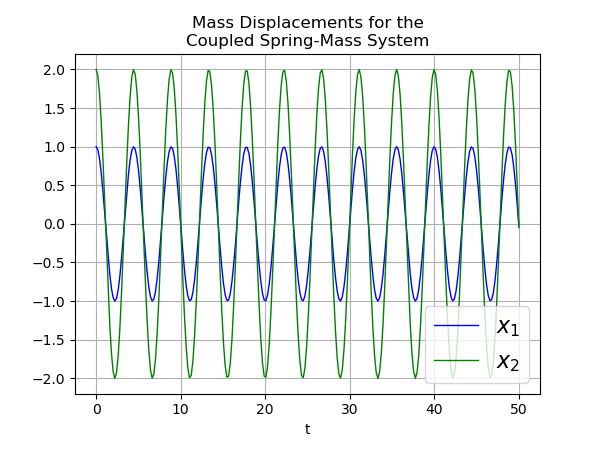
\includegraphics[width=9cm]{two_springs1-1.png}
 \end{center}





\begin{verbatim} 

%matplotlib inline

t, x1, xy, x2, y2, E1, E2 = loadtxt('two_springs1.dat', unpack=True)

figure(1, figsize=(6, 4.5))

grid(True)
lw = 1

plot(x1, x2, 'b', linewidth=lw)

legend((r'$x_1$', r'$x_2$'), prop=FontProperties(size=16))
title('x1 VS x2\nCoupled Spring-Mass System')
savefig('two_springs1-2.png', dpi=100)

\end{verbatim}


\begin{center}
 	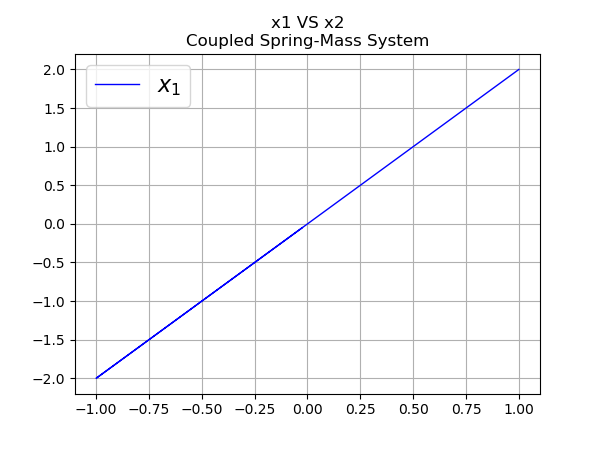
\includegraphics[width=9cm]{two_springs1-2.png}
 \end{center}


\begin{verbatim} 

%matplotlib inline

t, x1, xy, x2, y2, E1, E2 = loadtxt('two_springs1.dat', unpack=True)

figure(1, figsize=(6, 4.5))

grid(True)
lw = 1

plot(xy, x1, 'b', linewidth=lw)

plot(y2, x2, 'g', linewidth=lw)

legend((r'$x_1$', r'$x_2$'), prop=FontProperties(size=16))
title('x VS y\nCoupled Spring-Mass System')
savefig('two_springs1-3.png', dpi=100)

\end{verbatim}



\begin{center}
 	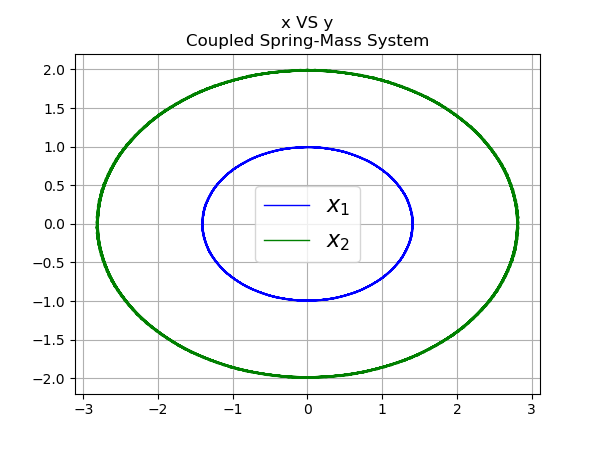
\includegraphics[width=9cm]{two_springs1-3.png}
 \end{center}



** Gráficas de error para valor calculado VS valor teórico.


\begin{verbatim} 

%matplotlib inline

t, x1, xy, x2, y2, E1, E2 = loadtxt('two_springs1.dat', unpack=True)

figure(1, figsize=(6, 4.5))

grid(True)
lw = 1

plot(t, E1, 'r', linewidth=lw)

legend((r'$x_1$', r'$x_2$'), prop=FontProperties(size=16))
title('Error 1')
savefig('two_springs1-E1.png', dpi=100)

\end{verbatim}



\begin{center}
 	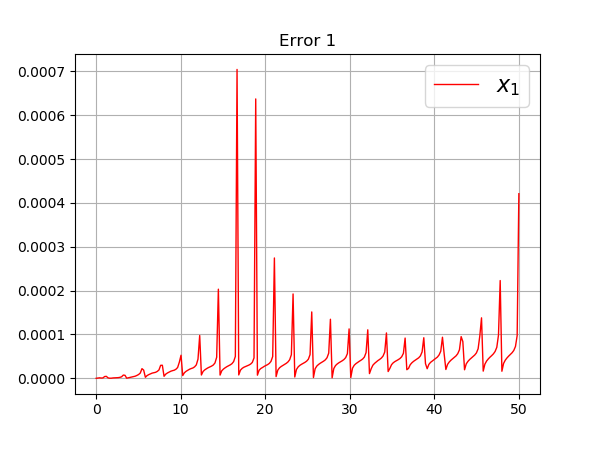
\includegraphics[width=9cm]{two_springs1-E1.png}
 \end{center}




\begin{verbatim} 

%matplotlib inline

t, x1, xy, x2, y2, E1, E2 = loadtxt('two_springs1.dat', unpack=True)

figure(1, figsize=(6, 4.5))

grid(True)
lw = 1

plot(t, E2, 'b', linewidth=lw)

legend((r'$x_1$', r'$x_2$'), prop=FontProperties(size=16))
title('Error 2')
savefig('two_springs1-E2.png', dpi=100)

\end{verbatim}



\begin{center}
 	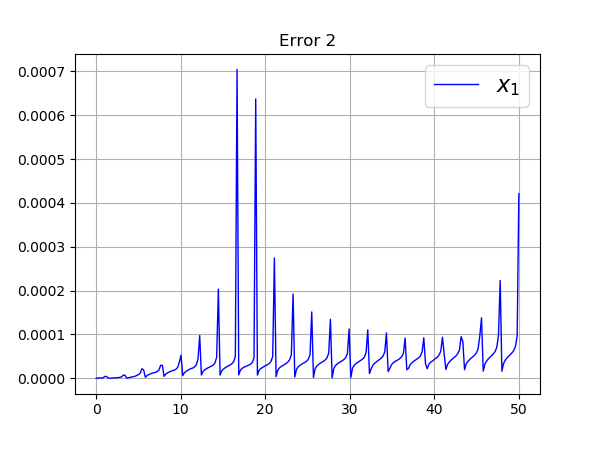
\includegraphics[width=9cm]{two_springs1-E2.png}
 \end{center}


\subsection{Ejemplo 2.2.}
Se describe el movimiento de dos resortes con constantes k1=6 y k2=4 con condiciones iniciales (-2,0,1,0).

\vspace{0.5 cm}

** Resolución con jupyter lab de las ecuaciones correspondientes:

\begin{verbatim} 

# Use ODEINT to solve the differential equations defined by the vector field
from scipy.integrate import odeint

# Parameter values
# Masses:
m1 = 1.0
m2 = 1.0

# Spring constants
k1 = 6.0
k2 = 4.0

# Natural lengths
L1 = 0.0
L2 = 0.0

# Friction coefficients
b1 = 0.0
b2 = 0.0

# Initial conditions
# x1 and x2 are the initial displacements; y1 and y2 are the initial velocities
x1 = -2.0
y1 = 0.0
x2 = 1.0
y2 = 0.0

# ODE solver parameters
abserr = 1.0e-8
relerr = 1.0e-6
stoptime = 25.0
numpoints = 250

# Create the time samples for the output of the ODE solver.
# I use a large number of points, only because I want to make
# a plot of the solution that looks nice.
t = [stoptime * float(i) / (numpoints - 1) for i in range(numpoints)]

# Pack up the parameters and initial conditions:
p = [m1, m2, k1, k2, L1, L2, b1, b2]
w0 = [x1, y1, x2, y2]

# Call the ODE solver.
wsol = odeint(vectorfield, w0, t, args=(p,),
              atol=abserr, rtol=relerr)

with open('two_springs2.dat', 'w') as f:
    # Print & save the solution.
    for t1, w1 in zip(t, wsol):
        print (t1, w1[0], w1[1], w1[2], w1[3], np.abs((-2.0*np.cos(2.0*np.sqrt(3.0)*t1)-w1[0])/(-2.0*np.cos(2.0*np.sqrt(3.0)*t1))), np.abs((np.cos(2.0*np.sqrt(3.0)*t1)-w1[2])/(np.cos(2.0*np.sqrt(3.0)*t1))), file=f)

\end{verbatim}

**Gráficas correspondientes al ejercicio 2.2:

\begin{verbatim} 

# Plot the solution that was generated

from numpy import loadtxt
from pylab import figure, plot, xlabel, grid, hold, legend, title, savefig
from matplotlib.font_manager import FontProperties
%matplotlib inline

t, x1, xy, x2, y2, E1, E2 = loadtxt('two_springs2.dat', unpack=True)

figure(1, figsize=(6, 4.5))

xlabel('t')
grid(True)
#hold(True)
lw = 1

plot(t, x1, 'b', linewidth=lw)
plot(t, x2, 'g', linewidth=lw)

legend((r'$x_1$', r'$x_2$'), prop=FontProperties(size=16))
title('Mass Displacements for the\nCoupled Spring-Mass System')
savefig('two_springs2-1.png', dpi=100)

\end{verbatim}



\begin{center}
 	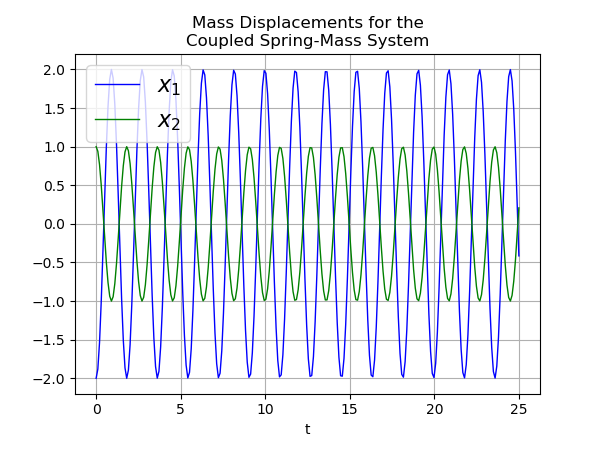
\includegraphics[width=9cm]{two_springs2-1.png}
 \end{center}





\begin{verbatim} 

%matplotlib inline

t, x1, xy, x2, y2, E1, E2 = loadtxt('two_springs2.dat', unpack=True)

figure(1, figsize=(6, 4.5))

grid(True)
lw = 1

plot(x1, x2, 'b', linewidth=lw)

legend((r'$x_1$', r'$x_2$'), prop=FontProperties(size=16))
title('x1 VS x2\nCoupled Spring-Mass System')
savefig('two_springs2-2.png', dpi=100)

\end{verbatim}


\begin{center}
 	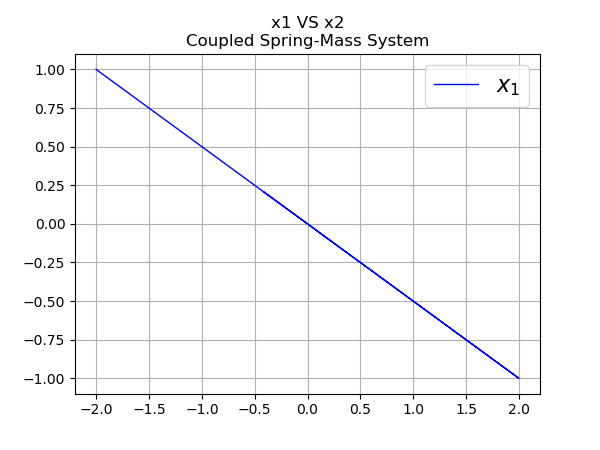
\includegraphics[width=9cm]{two_springs2-2.png}
 \end{center}


\begin{verbatim} 

%matplotlib inline

t, x1, xy, x2, y2, E1, E2 = loadtxt('two_springs2.dat', unpack=True)

figure(1, figsize=(6, 4.5))

grid(True)
lw = 1

plot(xy, x1, 'b', linewidth=lw)

plot(y2, x2, 'g', linewidth=lw)

legend((r'$x_1$', r'$x_2$'), prop=FontProperties(size=16))
title('x VS y\nCoupled Spring-Mass System')
savefig('two_springs2-3.png', dpi=100)

\end{verbatim}



\begin{center}
 	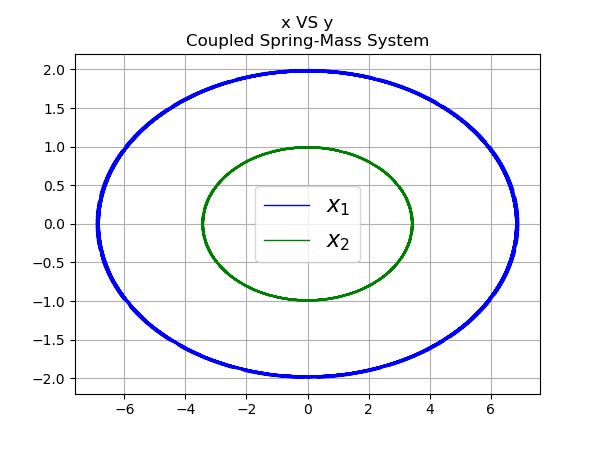
\includegraphics[width=9cm]{two_springs2-3.png}
 \end{center}



** Gráficas de error para valor calculado VS valor teórico.


\begin{verbatim} 

%matplotlib inline

t, x1, xy, x2, y2, E1, E2 = loadtxt('two_springs2.dat', unpack=True)

figure(1, figsize=(6, 4.5))

grid(True)
lw = 1

plot(t, E1, 'r', linewidth=lw)

legend((r'$x_1$', r'$x_2$'), prop=FontProperties(size=16))
title('Error 1')
savefig('two_springs2-E1.png', dpi=100)

\end{verbatim}



\begin{center}
 	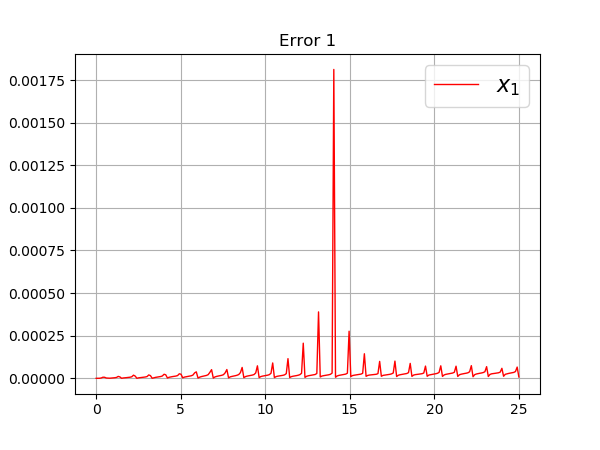
\includegraphics[width=9cm]{two_springs2-E1.png}
 \end{center}




\begin{verbatim} 

%matplotlib inline

t, x1, xy, x2, y2, E1, E2 = loadtxt('two_springs2.dat', unpack=True)

figure(1, figsize=(6, 4.5))

grid(True)
lw = 1

plot(t, E2, 'b', linewidth=lw)

legend((r'$x_1$', r'$x_2$'), prop=FontProperties(size=16))
title('Error 2')
savefig('two_springs2-E2.png', dpi=100)

\end{verbatim}



\begin{center}
 	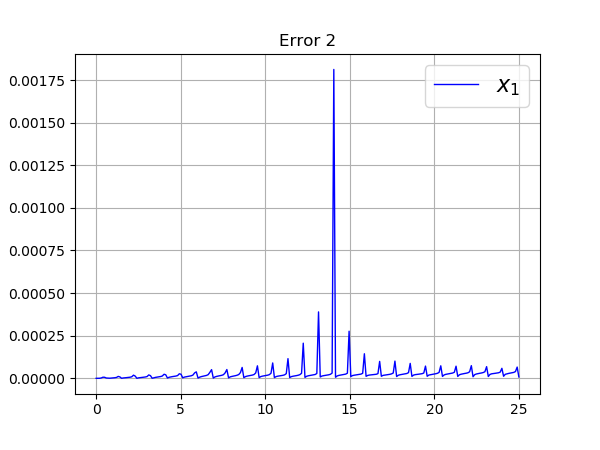
\includegraphics[width=9cm]{two_springs2-E2.png}
 \end{center}




\subsection{Ejemplo 2.3.}
Se describe el movimiento de dos resortes con constantes k1=0.4 y k2=1.808 con condiciones iniciales (1/2,0,-1/2,7/10).

\vspace{0.5 cm}

** Resolución con jupyter lab de las ecuaciones correspondientes:

\begin{verbatim} 

def vectorfield(w, t, p):
    """
    Defines the differential equations for the coupled spring-mass system.

    Arguments:
        w :  vector of the state variables:
                  w = [x1,y1,x2,y2]
        t :  time
        p :  vector of the parameters:
                  p = [m1,m2,k1,k2,L1,L2,b1,b2]
    """
    x1, y1, x2, y2 = w
    m1, m2, k1, k2, L1, L2, b1, b2 = p

    # Create f = (x1',y1',x2',y2'):
    f = [y1,(-b1 * y1 - k1 * (x1 - L1) + k2 * (x2 - x1 - L2)) / m1,y2,(-b2 * y2 - k2 * (x2 - x1 - L2)) / m2]
    return f


# Use ODEINT to solve the differential equations defined by the vector field
from scipy.integrate import odeint

# Parameter values
# Masses:
m1 = 1.0
m2 = 1.0

# Spring constants
k1 = 0.4
k2 = 1.808

# Natural lengths
L1 = 0.0
L2 = 0.0

# Friction coefficients
b1 = 0.0
b2 = 0.0

# Initial conditions
# x1 and x2 are the initial displacements; y1 and y2 are the initial velocities
x1 = 0.5
y1 = 0.0
x2 = -0.5
y2 = 7/10

# ODE solver parameters
abserr = 1.0e-8
relerr = 1.0e-6
stoptime = 50.0
numpoints = 250

# Create the time samples for the output of the ODE solver.
# I use a large number of points, only because I want to make
# a plot of the solution that looks nice.
t = [stoptime * float(i) / (numpoints - 1) for i in range(numpoints)]

# Pack up the parameters and initial conditions:
p = [m1, m2, k1, k2, L1, L2, b1, b2]
w0 = [x1, y1, x2, y2]

# Call the ODE solver.
wsol = odeint(vectorfield, w0, t, args=(p,), atol=abserr, rtol=relerr)

with open('two_springs3.dat', 'w') as f:
    # Print & save the solution.
    for t1, w1 in zip(t, wsol):
        print (t1, w1[0], w1[1], w1[2], w1[3], file=f)

\end{verbatim}


**Gráficas correspondientes al ejercicio 2.3:

\begin{verbatim} 

# Plot the solution that was generated

from numpy import loadtxt
from pylab import figure, plot, xlabel, grid, hold, legend, title, savefig
from matplotlib.font_manager import FontProperties
%matplotlib inline

t, x1, xy, x2, y2 = loadtxt('two_springs3.dat', unpack=True)

figure(1, figsize=(6, 4.5))

xlabel('t')
grid(True)
#hold(True)
lw = 1

plot(t, x1, 'b', linewidth=lw)
plot(t, x2, 'g', linewidth=lw)

legend((r'$x_1$', r'$x_2$'), prop=FontProperties(size=16))
title('Mass Displacements for the\nCoupled Spring-Mass System')
savefig('two_springs3-1.png', dpi=100)

\end{verbatim}



\begin{center}
 	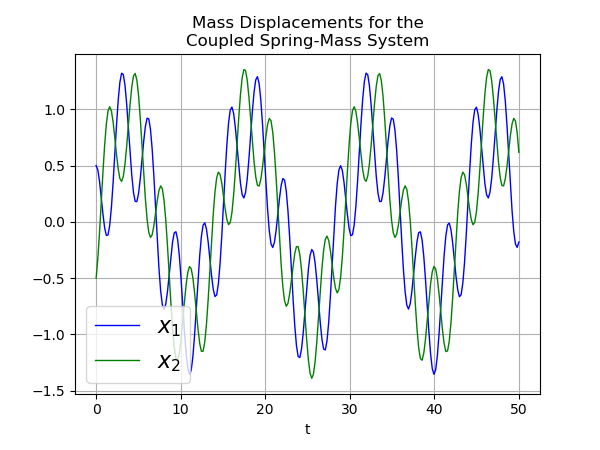
\includegraphics[width=9cm]{two_springs3-1.png}
 \end{center}



\begin{verbatim} 

%matplotlib inline

t, x1, xy, x2, y2 = loadtxt('two_springs3.dat', unpack=True)

figure(1, figsize=(6, 4.5))

grid(True)
lw = 1

plot(x1, x2, 'b', linewidth=lw)

legend((r'$x_1$', r'$x_2$'), prop=FontProperties(size=16))
title('x1 VS x2\nCoupled Spring-Mass System')
savefig('two_springs3-2.png', dpi=100)

\end{verbatim}


\begin{center}
 	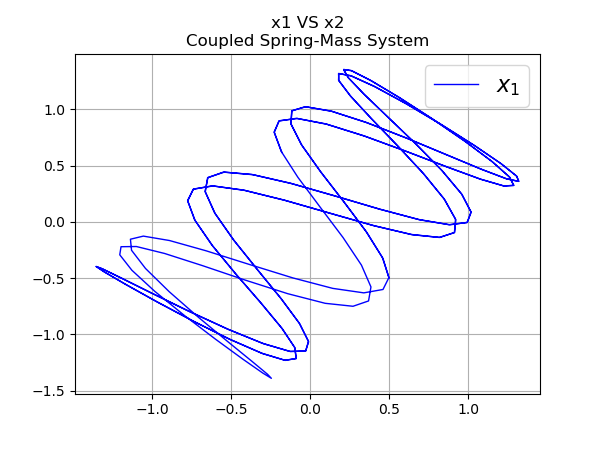
\includegraphics[width=9cm]{two_springs3-2.png}
 \end{center}


\begin{verbatim} 

%matplotlib inline

t, x1, xy, x2, y2 = loadtxt('two_springs3.dat', unpack=True)

figure(1, figsize=(6, 4.5))

grid(True)
lw = 1

plot(x1, xy, 'b', linewidth=lw)

legend((r'$x_1$', r'$x_2$'), prop=FontProperties(size=16))
title('x VS y\nCoupled Spring-Mass System')
savefig('two_springs3-3.png', dpi=100)

\end{verbatim}



\begin{center}
 	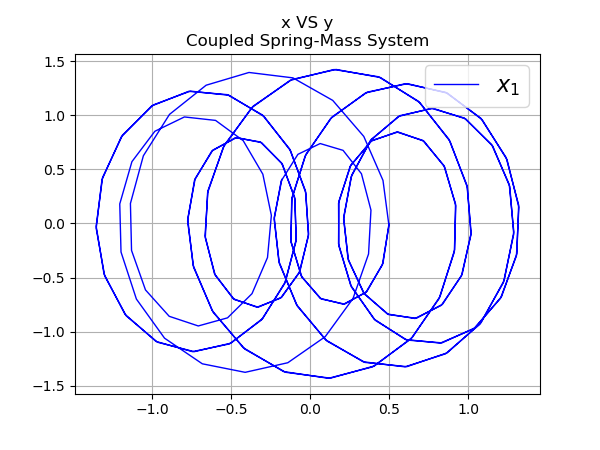
\includegraphics[width=9cm]{two_springs3-3.png}
 \end{center}



\begin{verbatim} 

%%matplotlib inline

t, x1, xy, x2, y2 = loadtxt('two_springs3.dat', unpack=True)

figure(1, figsize=(6, 4.5))

grid(True)
lw = 1

plot(x2, y2, 'g', linewidth=lw)

legend((r'$x_1$', r'$x_2$'), prop=FontProperties(size=16))
title('x VS y\nCoupled Spring-Mass System')
savefig('two_springs3-4.png', dpi=100)

\end{verbatim}



\begin{center}
 	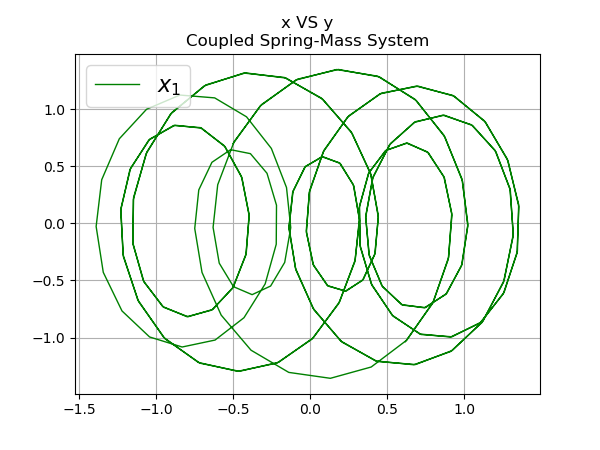
\includegraphics[width=9cm]{two_springs3-4.png}
 \end{center}


\subsection{Ejemplo 2.4.}
Se describe el movimiento de dos resortes con constantes k1=0.4 y k2=1.808 con condiciones iniciales (1,1/2,2,1/2) y coeficientes de fricción b1=0.1 y b2=0.2.

\vspace{0.5 cm}

** Resolución con jupyter lab de las ecuaciones correspondientes:

\begin{verbatim} 

def vectorfield(w, t, p):
    """
    Defines the differential equations for the coupled spring-mass system.

    Arguments:
        w :  vector of the state variables:
                  w = [x1,y1,x2,y2]
        t :  time
        p :  vector of the parameters:
                  p = [m1,m2,k1,k2,L1,L2,b1,b2]
    """
    x1, y1, x2, y2 = w
    m1, m2, k1, k2, L1, L2, b1, b2 = p

    # Create f = (x1',y1',x2',y2'):
    f = [y1,(-b1 * y1 - k1 * (x1 - L1) + k2 * (x2 - x1 - L2)) / m1,y2,(-b2 * y2 - k2 * (x2 - x1 - L2)) / m2]
    return f

# Use ODEINT to solve the differential equations defined by the vector field
from scipy.integrate import odeint

# Parameter values
# Masses:
m1 = 1.0
m2 = 1.0

# Spring constants
k1 = 0.4
k2 = 1.808

# Natural lengths
L1 = 0.0
L2 = 0.0

# Friction coefficients
b1 = 0.1
b2 = 0.2

# Initial conditions
# x1 and x2 are the initial displacements; y1 and y2 are the initial velocities
x1 = 1.0
y1 = 0.5
x2 = 2.0
y2 = 0.5

# ODE solver parameters
abserr = 1.0e-8
relerr = 1.0e-6
stoptime = 50.0
numpoints = 250

# Create the time samples for the output of the ODE solver.
# I use a large number of points, only because I want to make
# a plot of the solution that looks nice.
t = [stoptime * float(i) / (numpoints - 1) for i in range(numpoints)]

# Pack up the parameters and initial conditions:
p = [m1, m2, k1, k2, L1, L2, b1, b2]
w0 = [x1, y1, x2, y2]

# Call the ODE solver.
wsol = odeint(vectorfield, w0, t, args=(p,), atol=abserr, rtol=relerr)

with open('two_springs4.dat', 'w') as f:
    # Print & save the solution.
    for t1, w1 in zip(t, wsol):
        print (t1, w1[0], w1[1], w1[2], w1[3], file=f) 

\end{verbatim}


**Gráficas correspondientes al ejercicio 2.4:

\begin{verbatim} 

# Plot the solution that was generated

from numpy import loadtxt
from pylab import figure, plot, xlabel, grid, hold, legend, title, savefig
from matplotlib.font_manager import FontProperties
%matplotlib inline

t, x1, xy, x2, y2 = loadtxt('two_springs4.dat', unpack=True)

figure(1, figsize=(6, 4.5))

xlabel('t')
grid(True)
#hold(True)
lw = 1

plot(t, x1, 'b', linewidth=lw)
plot(t, x2, 'g', linewidth=lw)

legend((r'$x_1$', r'$x_2$'), prop=FontProperties(size=16))
title('Mass Displacements for the\nCoupled Spring-Mass System')
savefig('two_springs4-1.png', dpi=100)

\end{verbatim}



\begin{center}
 	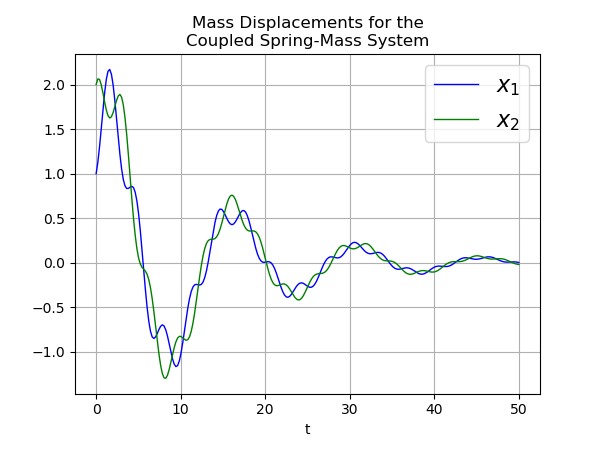
\includegraphics[width=9cm]{two_springs4-1.png}
 \end{center}



\begin{verbatim} 

%matplotlib inline

t, x1, xy, x2, y2 = loadtxt('two_springs4.dat', unpack=True)

figure(1, figsize=(6, 4.5))

grid(True)
lw = 1

plot(x1, x2, 'b', linewidth=lw)

legend((r'$x_1$', r'$x_2$'), prop=FontProperties(size=16))
title('x1 VS x2\nCoupled Spring-Mass System')
savefig('two_springs4-2.png', dpi=100)

\end{verbatim}


\begin{center}
 	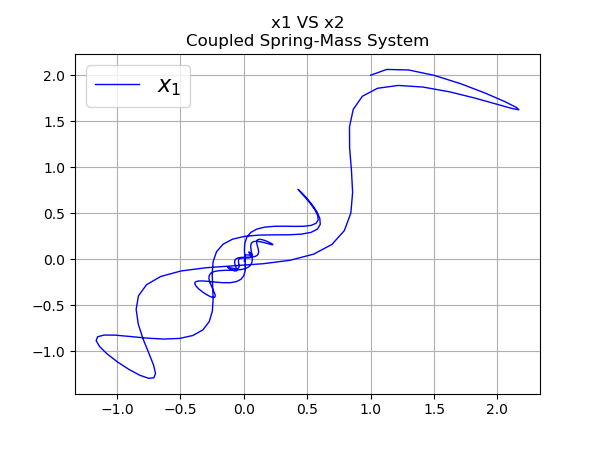
\includegraphics[width=9cm]{two_springs4-2.png}
 \end{center}


\begin{verbatim} 

%matplotlib inline

t, x1, xy, x2, y2 = loadtxt('two_springs4.dat', unpack=True)

figure(1, figsize=(6, 4.5))

grid(True)
lw = 1

plot(x1, xy, 'b', linewidth=lw)

legend((r'$x_1$', r'$x_2$'), prop=FontProperties(size=16))
title('x VS y\nCoupled Spring-Mass System')
savefig('two_springs4-3.png', dpi=100)

\end{verbatim}



\begin{center}
 	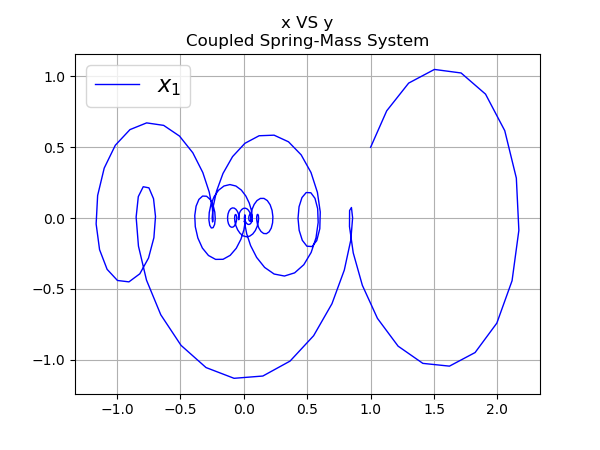
\includegraphics[width=9cm]{two_springs4-3.png}
 \end{center}



\begin{verbatim} 

%%matplotlib inline

t, x1, xy, x2, y2 = loadtxt('two_springs4.dat', unpack=True)

figure(1, figsize=(6, 4.5))

grid(True)
lw = 1

plot(x2, y2, 'g', linewidth=lw)

legend((r'$x_1$', r'$x_2$'), prop=FontProperties(size=16))
title('x VS y\nCoupled Spring-Mass System')
savefig('two_springs4-4.png', dpi=100)

\end{verbatim}



\begin{center}
 	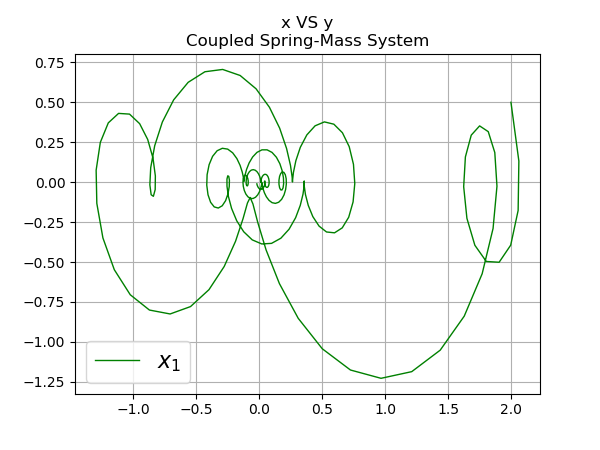
\includegraphics[width=9cm]{two_springs4-4.png}
 \end{center}

\vspace{12 cm}

\section*{Apéndice}

\hspace{0.45 cm} ¿En general te pareció interesante esta actividad de modelación matemática? ¿Qué te gustó mas? ¿Qué no te gustó?

\vspace{0.5 cm}

** La actividad fué muy interesante pues nos expuso al ambiente de Jupyter lab y nuevas posibilidades de manejo matemático de datos. Me gustó la parte gráfica de la actividad.

\vspace{0.5 cm}

La cantidad de material te pareció ¿bien?, ¿suficiente?, ¿demasiado?

\vspace{0.5 cm}

** La cantidad de material fué adecuada para los propósitos de aprendizaje de la sesión sin llegar a ser excesiva. 

\vspace{0.5 cm}

¿Cuál es tu primera impresión de Jupyter Lab? 

\vspace{0.5 cm}

** Al igual que Jupyter Notebook es un ambiente muy amigable con el usuario que de manera rápida se comienza a utilizar fluida y cómodamente. 

\vspace{0.5 cm}

Respecto al uso de funciones de SciPy, ¿ya habías visto integración numérica en tus cursos anteriores? ¿Cuál es tu experiencia?.

\vspace{0.5 cm}

** Esta es la primera vez que se lleva a cabo un ejercicio de este tipo. 

\vspace{0.5 cm}

El tema de sistema de masas acopladas con resortes, ¿ya lo habías resuelto en tu curso de Mecánica 2?  

\vspace{0.5 cm}

** Si, el problema se aborda desde una perspectiva idealizada y simplificada en los cursos de mecánica.

\vspace{0.5 cm}

¿Qué le quitarías o agregarías a esta actividad para hacerla más interesante y divertida? 

\vspace{0.5 cm}

** No le agregaría ni quitaría nada pues me pareció muy adecuada. 

\vspace{0.5 cm}



\end{document}